\documentclass[journal, a4paper]{IEEEtran}

\usepackage{graphicx}
\usepackage{url}
\usepackage{bm}
\usepackage{amsmath}
\usepackage{amssymb}
\usepackage[justification=centering]{caption}
\usepackage{caption}
% Your document starts here!
\begin{document}
\begin{titlepage}

\newcommand{\HRule}{\rule{\linewidth}{0.5mm}} % Defines a new command for the horizontal lines, change thickness here

\center % Center everything on the page
 %----------------------------------------------------------------------------------------
%	LOGO SECTION
%----------------------------------------------------------------------------------------

~\\[1cm]

\includegraphics{SCUT.png}\\[2cm] % Include a department/university logo - this will require the graphicx package

%----------------------------------------------------------------------------------------
%	TITLE SECTION
%----------------------------------------------------------------------------------------

\HRule \\[1cm]
{ \huge \bfseries The Experiment Report of \textit{Deep Learning} }\\[0.6cm] % Title of your document
\HRule \\[2cm]
%----------------------------------------------------------------------------------------
%	HEADING SECTIONS
%----------------------------------------------------------------------------------------


\textsc{\LARGE \textbf{School:} School of Software Engineering}\\[1cm]
\textsc{\LARGE \textbf{Subject:} Software Engineering}\\[2cm]


%----------------------------------------------------------------------------------------
%	AUTHOR SECTION
%----------------------------------------------------------------------------------------

\begin{minipage}{0.4\textwidth}
\begin{flushleft} \large
\emph{Author:}\\
Qichen Huang % Your name
\end{flushleft}
\end{minipage}
~
\begin{minipage}{0.4\textwidth}
\begin{flushright} \large
\emph{Supervisor:} \\
Mingkui Tan% Supervisor's Name
\end{flushright}
\end{minipage}\\[2cm]
~
\begin{minipage}{0.4\textwidth}
\begin{flushleft} \large
\emph{Student ID:}\\
201920142806
\end{flushleft}
\end{minipage}
~
\begin{minipage}{0.4\textwidth}
\begin{flushright} \large
\emph{Grade:} \\
Graduate
\end{flushright}
\end{minipage}\\[2cm]

% If you don't want a supervisor, uncomment the two lines below and remove the section above
%\Large \emph{Author:}\\
%John \textsc{Smith}\\[3cm] % Your name

%----------------------------------------------------------------------------------------
%	DATE SECTION
%----------------------------------------------------------------------------------------

{\large \today}\\[2cm] % Date, change the \today to a set date if you want to be precise


%----------------------------------------------------------------------------------------

\vfill % Fill the rest of the page with whitespace

\end{titlepage}

% Define document title and author
	\title{Face Detection Based on MTCNN}
	\maketitle

% Write abstract here
\begin{abstract}
Face detection is a detection problem for human faces and it plays an important role in downstream tasks, like face recognition.
Since MTCNN is known as a powerful model for solving face detection problem, we explore its structure details and try to reimplement it.
After three-stage cascaded network training, we finally obtain a well-perform model which can exactly predict bounding boxes and landmarks' positions.
\end{abstract}

% Each section begins with a \section{title} command
\section{Introduction}
	% \PARstart{}{} creates a tall first letter for this first paragraph
\PARstart{F}{ace} detection is a kind of object detection problem, whose target is to detection an object, such as cars, pedestrians and cyclists.
As its name suggests, face detection focusses on human faces detection.
Concretely, it draws a rectangle, named as bounding box, in a given picture to exactly include a human face.
Since face detection helps to concentrate computation resources on the detected bounding box, it is the first and essential procedure in face recognition.

Due to powerful strength of deep learning, recent researches on face detection are based on deep neural network.
In this experiment, we handle face detection task using Multi-task Convolutional Neural Networks(MTCNN), proposed by Kaipeng Zhang.

Our motivation is to 1) understand the basic theory of face detection using neural network, 2) understand the processes of MTCNN and use it in practice.
% Main Part
\section{Methods and Theory}
The MTCNN model that we use in this experiment, proposed by Kaipeng Zhang et al, explores the relationship between face detection and face alignment and integrate these two task using unified cascaded CNNs by multi-task learning.

The CNN architectures are shown in Fig. \ref{fig:CNN_architecture}.
\begin{figure}[!hbt]
	\begin{center}
	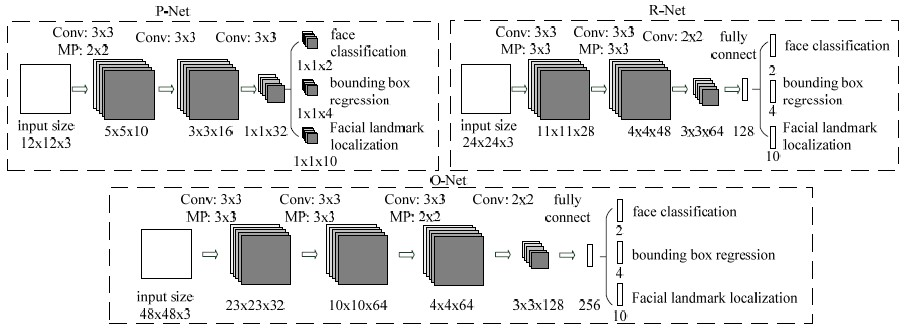
\includegraphics[width=\columnwidth]{CNN_architecture}
    \captionsetup{font={scriptsize}}
	\caption{The architectures of P-Net, R-Net, and O-Net, where ��MP�� means max pooling and ��Conv�� means convolution.
        The step size in convolution and pooling is 1 and 2, respectively.}
	\label{fig:CNN_architecture}
	\end{center}
\end{figure}
PReLU is used as nonlinearity activation function after the convolution and fully connection layers (except output layers).

The CNN detectors are then trained leveraging three tasks: face/non-face classification, bounding box regression, and facial landmark localization.

In face classification task, the learning objective is formulated as a two-class classification problem. For each sample $x_i$, we use the cross-entropy loss:
\begin{equation}
L_i^{det}=-(y_i^{det}\log(p_i)+(1-y_i^{det})(1-\log(p_i)))
\end{equation}
where $p_i$ is the probability produced by the network that indicates sample $x_i$ being a face.
The notation $y_i^{det} \in \{0,1\}$ denotes the ground-truth label.

In bounding box regression, for each candidate window, we predict the offset between it and the nearest ground truth (i.e., the bounding boxes�� left, top, height, and width).
The learning objective is formulated as a regression problem, and we employ the Euclidean loss for each sample $x_i$:
\begin{equation}
L_i^{box}=||\hat{y}_i^{box}-y_i^{box}||_2^2
\end{equation}
where $\hat{y}_i^{box}$ is the regression target obtained from the network and $y_i^{box}$ is the ground-truth coordinate.
There are four coordinates, including left top, height and width, and thus $y_i^{box} \in \mathbb{R}^4$

In facial landmark localization, similar to bounding box regression task, facial landmark detection is formulated as a
regression problem and we minimize the Euclidean loss:
\begin{equation}
L_i^{landmark}=||\hat{y}_i^{landmark}-y_i^{landmark}||_2^2
\end{equation}
where $\hat{y}_i^{landmark}$ is the facial landmark��s coordinates obtained from the network and $y_i^{landmark}$ is the ground-truth coordinate for the i-th sample.
There are five facial landmarks, including left eye, right eye, nose, left mouth corner, and right mouth corner, and thus $y_i^{landmark} \in \mathbb{R}^{10}$

\section{Experiments}
\subsection{Dataset}
For training MTCNN model, we utilize different image data on different training tasks.
When training PNet and Rnet, we use WiderFace, for face classification and face bounding box regression.
When training ONet, we use Wider Face for face classification and face bounding box regression, and use \textit{CNN for Facial Point Detection} Training Dataset for face feature point regression.
WIDER FACE dataset consists of 393,703 labeled face bounding boxes in 32,203 images and Facial Point Detection dataset contains 5,590 LFW images and 7,876 other images downloaded from the web.

Since MTCNN model jointly perform face detection and alignment, we use four different kinds of data annotation in our training
process: (i) Negatives: Regions whose the Intersection-over-Union (IoU) ratio are less than 0.3 to any ground-truth faces; (ii) Positives: IoU above 0.65 to a ground truth face; (iii) Part faces: IoU between 0.4 and 0.65 to a ground truth face; and (iv) Landmark faces: faces labeled 5 landmarks�� positions.Negatives and positives are used for face classification tasks, positives and part faces are used for bounding box regression, and landmark faces are used for facial landmark localization. The training data collection for each network is described as follows:
\begin{enumerate}
  \item \textit{P-Net:} We randomly crop several patches from WIDER FACE to collect positives, negatives and part face.
  \item \textit{R-Net:} We use the first stage of MTCNN to detect faces from WIDER FACE to collect positives, negatives and part face
  \item \textit{O-Net:} Similar to R-Net to collect data but we use the first two stages of our framework to detect faces and collect face classification and bounding box regression data. Then we randomly shift ground truth bounding boxes and crop landmark localization data.
\end{enumerate}

\subsection{Implementation}
The overall pipeline of MTCNN is shown in Fig. \ref{fig:overall_framework}.
\begin{figure}[!hbt]
	\begin{center}
	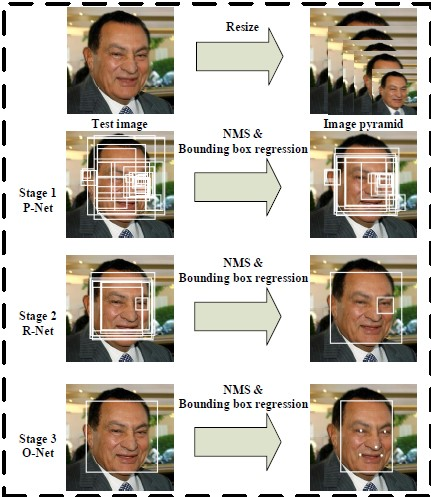
\includegraphics[width=\columnwidth]{overall_framework}
    \captionsetup{font={scriptsize}}
	\caption{Pipeline of MTCNN that includes three-stage multi-task deep convolutional networks.
        Firstly, candidate windows are produced through a fast Proposal Network (P-Net).
        After that, we refine these candidates in the next stage through a Refinement Network (R-Net).
        In the third stage, the Output Network (O-Net) produces final bounding box and facial landmarks position.}
	\label{fig:overall_framework}
	\end{center}
\end{figure}

Given an image, we initially resize it to different scales to build an image pyramid, which is the input of the following
three-stage cascaded framework:

\textbf{Stage 1:} We first exploit a fully convolutional network, called Proposal Network (P-Net), filtered with scores to obtain the candidate facial windows and their bounding box regression vectors.
Then candidates are calibrated based on the estimated bounding box regression vectors.
After that, we employ non-maximum suppression(NMS) to merge highly overlapped candidates.

\textbf{Stage 2:} All candidates are fed to another CNN, called Refine Network (R-Net), which further rejects a large number of
false candidates, performs calibration with bounding box regression, and conducts NMS.

\textbf{Stage 3:} This stage is similar to the second stage, but in this stage we aim to identify face regions with more supervision.
Besides candidates obtained from previous network, we also apply landmark localization data to help training a final CNN, called Output Network (O-Net), which will output bounding boxes as well as five facial landmarks�� positions.

\section{Conclusion}
In this paper, we briefly introduce face detection problem at first.
Then we reveal the details of architecture of MTCNN model.
After that, we present the generation of network input data and the procedures of how the model works.
Thanks to the help of MTCNN model, we now can correctly predict facial landmarks' positions in most cases.

% Your document ends here!
\end{document}
